\section{Promoting Evolvability in EANN} \label{sec:eann}

\begin{frame}{HyperNEAT}
\begin{figure}
	 \begin{tikzpicture}
    \node (first) {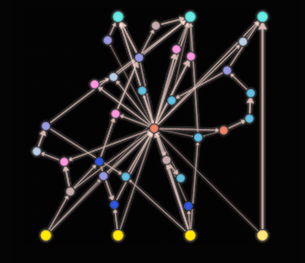
\includegraphics[width=0.25\textwidth]{img/cppn}};
    \node (second) [right=of first] {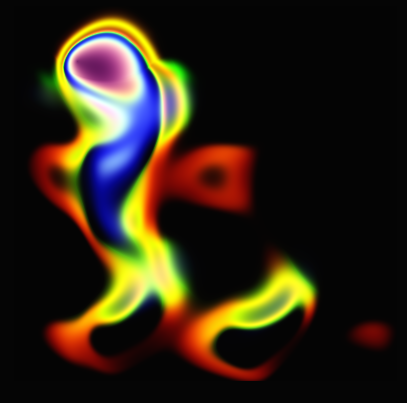
\includegraphics[width=0.25\textwidth]{img/walking_fish}};
    \node (third) [right=of second] {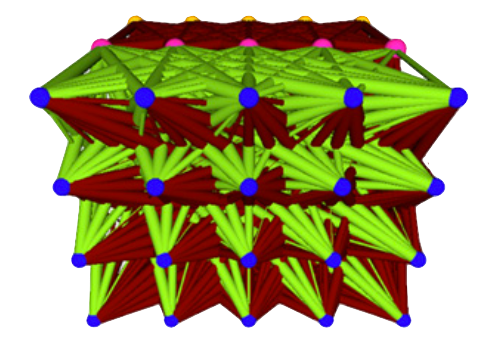
\includegraphics[width=0.25\textwidth]{img/neural_network}};

    \node (a) [right=of first] {};
    \node (b) [left=of second] {};
    \node (c) [right=of second] {};
    \node (d) [left=of third] {};

    \draw [ultra thick,->] (b) to (a);
    \draw [ultra thick,->] (d) to (c);
\end{tikzpicture}
    \captionsetup{singlelinecheck=off,justification=raggedright}
    \vspace{-4ex}
  	\caption{The working principle of HyperNEAT indirect genetic encoding; the genotype, a Compositional Pattern Producing Network (left), is used to construct a neural network configuration (right) \cite{Ha2015Neurogram}, \cite[Figure 15]{Clune2011OnRegularity}}
\end{figure}
\end{frame}

\begin{frame}{Novelty Search}
   \begin{figure}
  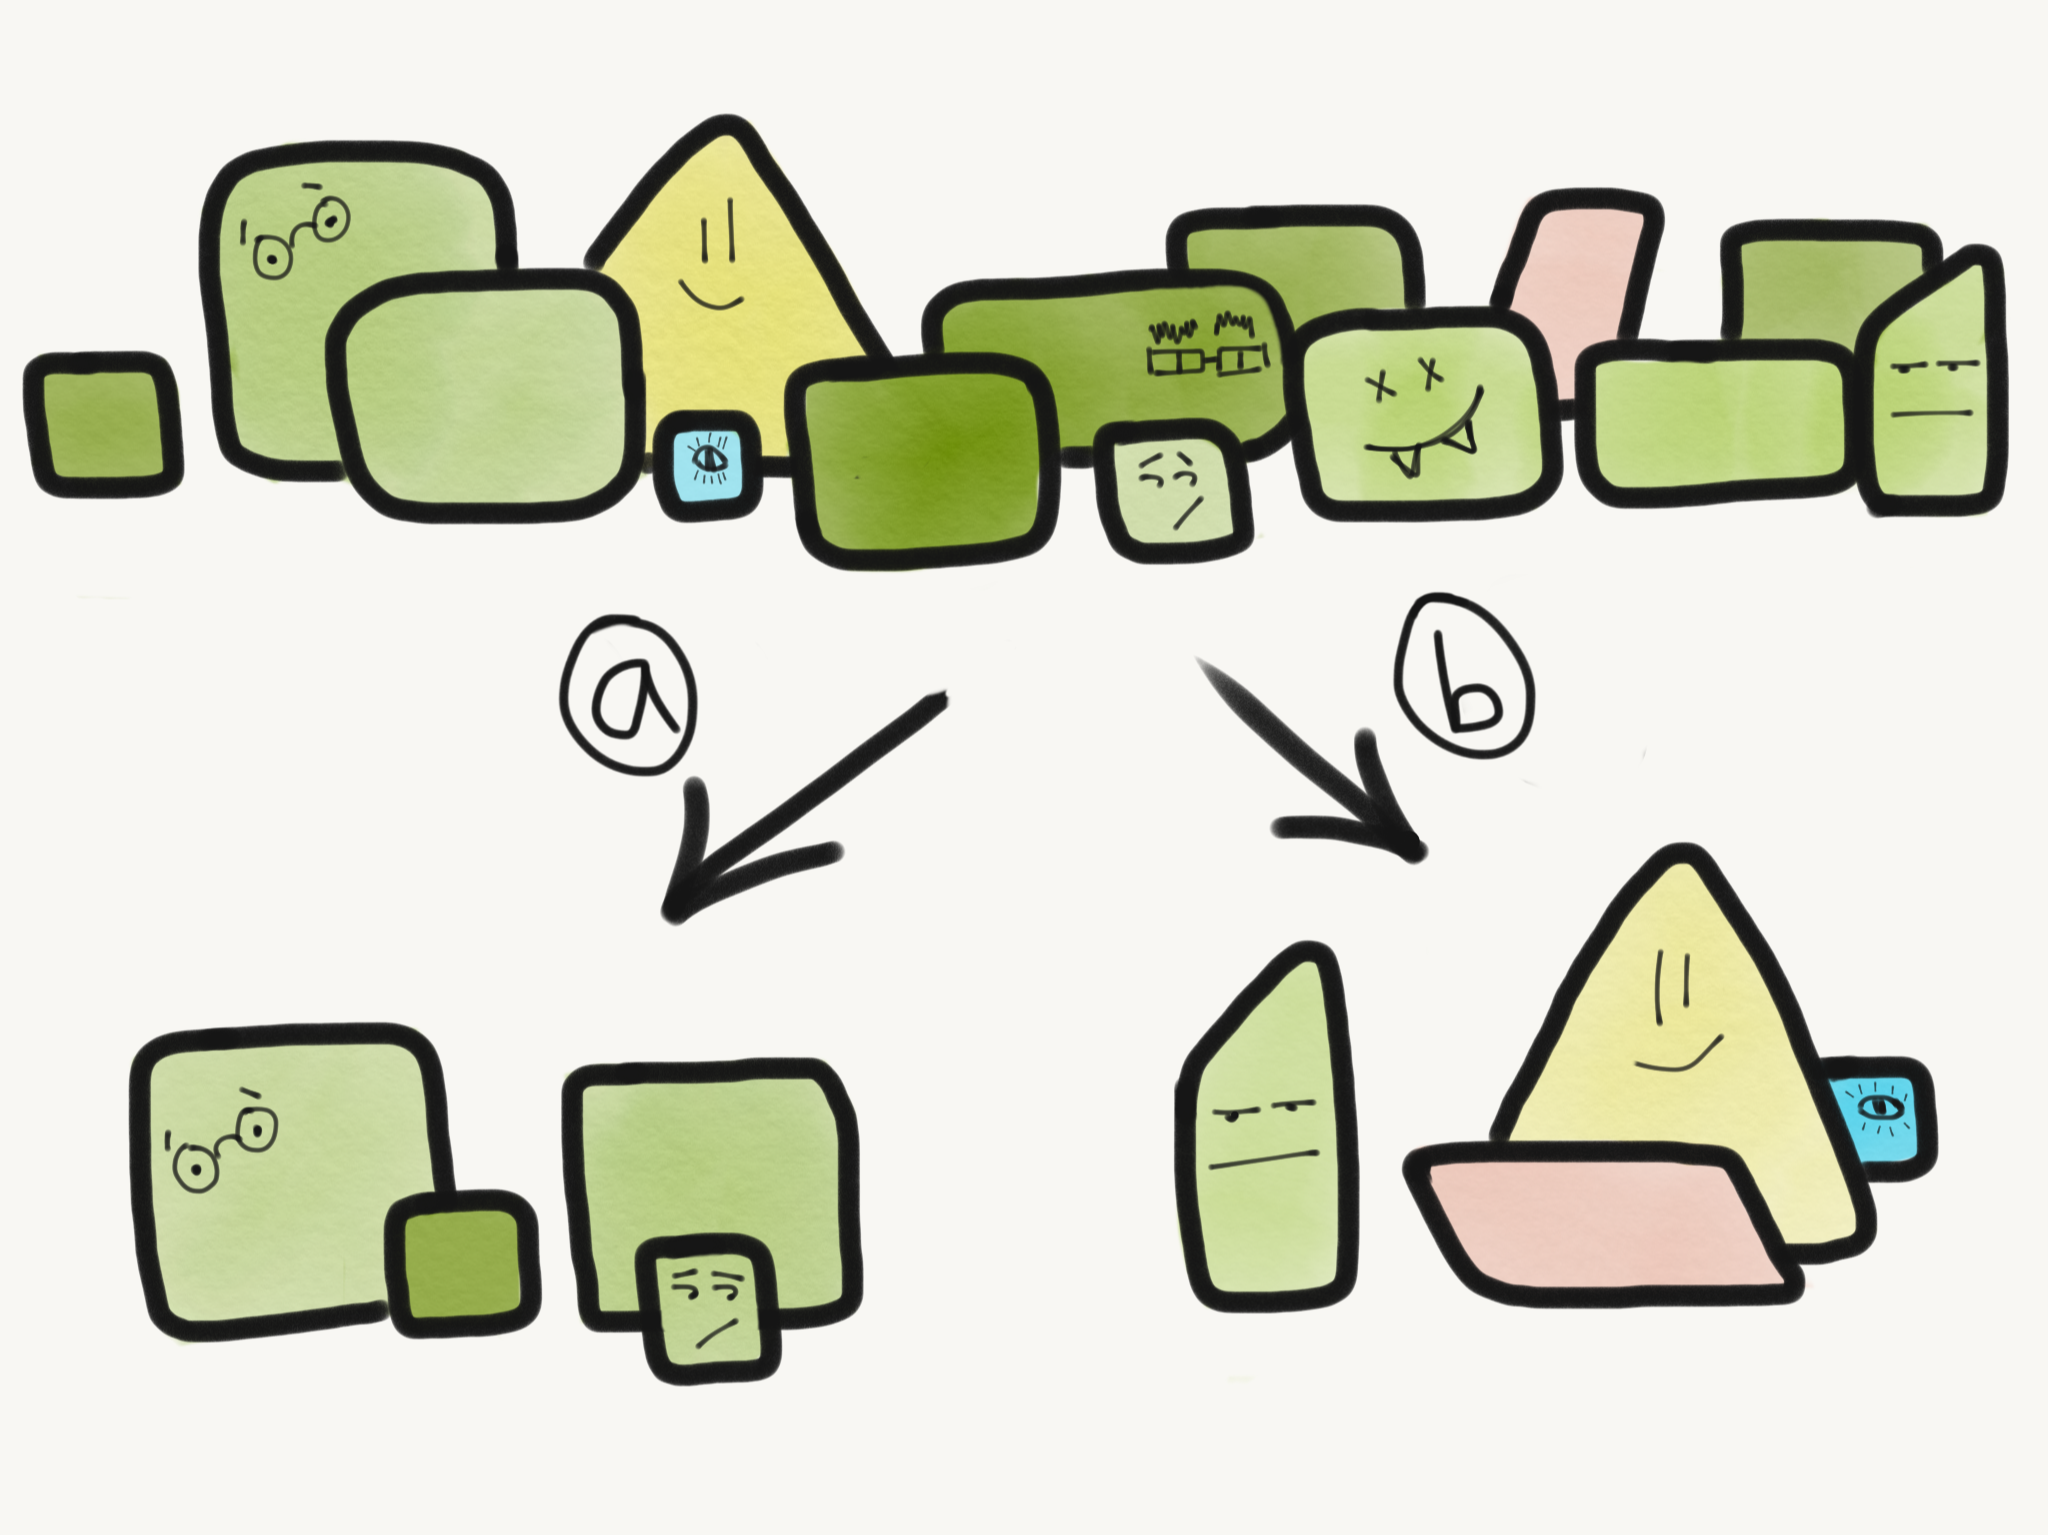
\includegraphics[width=0.8\textwidth]{img/novelty_search}
  \captionsetup{singlelinecheck=off,justification=raggedright}
  \caption{Novelty search, an example of divergent selection \cite{Wilder2015ReconcilingEvolvability}}
\end{figure}
\end{frame}